\chapter{Полугруппы, моноиды, группы, кольца и поля}\label{chap:c22}\markright{Глава 33}

\section{Одинаковые правила в разных множествах}
\par\addvspace{5pt}\begin{lrbox}{\CatFlowBox}\begin{minipage}[t]{\linewidth}
\setlength{\parskip}{5pt}\setlength{\columnsep}{4.5mm}\setlength{\intextsep}{0pt}
\begin{wrapfigure}[12]{r}{54mm}

\includegraphics[width=54mm,height=58mm,keepaspectratio]{images/unique/art-63.png}
\label{catflow:63}
\end{wrapfigure}
В главе \ref{chap:c01} мы перечислили свойства действий с рациональными числами. Теперь можно дать названия наборам этих свойств. Например, сложение целых чисел, сложение векторов и последовательное выполнение сдвигов устроены во многом одинаково: есть нейтральное действие, каждое действие можно отменить, а скобки можно переставлять. Такой общий язык позволяет однажды доказать правило и затем применять его в разных примерах.
\par\WFclear\end{minipage}\end{lrbox}%
\ifdim\dimexpr\ht\CatFlowBox+\dp\CatFlowBox\relax<64mm\dp\CatFlowBox=\dimexpr64mm-\ht\CatFlowBox\relax\fi%
\noindent\usebox{\CatFlowBox}\par\addvspace{5pt}
\begin{definition}
\term{Бинарная операция} (binary operation) на непустом множестве \(S\) — отображение \(*:S\times S\to S\), сопоставляющее каждой упорядоченной паре элементов единственный элемент \(a*b\) того же множества. Требование результата в \(S\) называют \term{замкнутостью} (closure).
\end{definition}
Сложение — операция на \(\mathbb N_0\), а вычитание — нет: \(1-2\notin\mathbb N_0\). На \(\mathbb Z\) вычитание уже замкнуто. Поэтому свойство действия всегда проверяют вместе с множеством, на котором оно задано. Обозначение \(*\) не обязательно означает обычное умножение.

\begin{definition}
Операция \term{ассоциативна} (associative), если \((a*b)*c=a*(b*c)\) для любых \(a,b,c\in S\). Она \term{коммутативна} (commutative), если \(a*b=b*a\) для любых \(a,b\in S\). Элемент \(e\in S\) — \term{нейтральный элемент} (identity element), если \(e*a=a*e=a\) для любого \(a\in S\).
\end{definition}
Ассоциативность разрешает опускать скобки в произведении нескольких элементов. Коммутативность разрешает переставлять сами элементы; это другое свойство. При композиции функций порядок обычно важен, даже когда скобки можно менять.

\section{Полугруппа, моноид и группа}
\begin{definition}
\term{Полугруппа} (semigroup) — непустое множество с ассоциативной бинарной операцией. \term{Моноид} (monoid) — полугруппа с нейтральным элементом.
\end{definition}
Положительные натуральные числа со сложением образуют полугруппу, но не моноид: нужного нейтрального числа \(0\) в \(\mathbb N\) нет. Множество \(\mathbb N_0\) со сложением — моноид. Все конечные слова над заданным алфавитом с операцией приписывания одного слова к другому тоже образуют моноид; его нейтральный элемент — пустое слово. Приписывание некоммутативно: слова «кот» и «ток» после приписывания дадут разные результаты в разном порядке.

\begin{definition}
В моноиде элемент \(b\) — \term{обратный элемент} (inverse element) к \(a\), если \(a*b=b*a=e\). \term{Группа} (group) — моноид, в котором у каждого элемента есть обратный. \term{Абелева группа} (abelian group) — группа с коммутативной операцией.
\end{definition}
Для сложения нейтральный элемент обычно обозначают \(0\), обратный к \(a\) — \(-a\). Для умножения используют \(1\) и \(a^{-1}\). Это выбор записи: в абстрактной группе знак \(a^{-1}\) не обязан означать привычную дробь.

Примеры абелевых групп: \((\mathbb Z,+)\), \((\mathbb Q,+)\), \((\mathbb R^2,+)\); также \((\mathbb Q\setminus\{0\},\cdot)\). Моноид \((\mathbb N_0,+)\) не является группой: у \(1\) нет противоположного внутри \(\mathbb N_0\). Все рациональные числа с умножением тоже не группа: у нуля нет обратного. По модулю \(m\ge2\) все классы образуют абелеву группу по сложению, причём противоположный к \([a]_m\) равен \([-a]_m\).

\begin{theorem}[Единственность нейтрального и обратного]\label{thm:legacy-c22-1}
Нейтральный элемент моноида единственен. Обратный элемент к заданному элементу, если он существует, также единственен.
\end{theorem}
\begin{proof}
Если \(e,f\) оба нейтральны, то \(e*f=f\) по свойству \(e\), но \(e*f=e\) по свойству \(f\). Значит, \(e=f\). Если \(b,c\) обратны к \(a\), то
\[
b=b*e=b*(a*c)=(b*a)*c=e*c=c.
\]
Равенство посередине использует ассоциативность, а не перестановку элементов. Это важно для некоммутативных групп.
\end{proof}

\begin{theorem}[Сокращение и решение уравнения в группе]\label{thm:legacy-c22-2}
В группе из \(a*b=a*c\) следует \(b=c\), а из \(b*a=c*a\) также следует \(b=c\). Уравнения \(a*x=b\) и \(y*a=b\) имеют единственные решения
\[
x=a^{-1}*b,\qquad y=b*a^{-1}.
\]
\end{theorem}
\begin{proof}
Первое равенство умножим слева на \(a^{-1}\), затем перегруппируем скобки: \((a^{-1}*a)*b=(a^{-1}*a)*c\), то есть \(b=c\). Во втором случае умножим справа. Эти же преобразования показывают необходимость формул для \(x,y\), а обратная подстановка подтверждает, что они дают решения. В некоммутативной группе место множителя \(a^{-1}\) менять нельзя.
\end{proof}

\section{Композиции и симметрии}
\begin{definition}
\term{Тождественное отображение} (identity map) множества \(X\) — отображение \(\operatorname{id}_X(x)=x\). \term{Перестановка множества} (permutation of a set) — биекция \(X\to X\). Все перестановки \(X\) образуют множество \(\operatorname{Sym}(X)\); для \(X=\{1,\ldots,n\}\) пишут также \(S_n\).
\end{definition}

\begin{theorem}[Группа перестановок]\label{thm:legacy-c22-3}
Множество \(\operatorname{Sym}(X)\) является группой относительно композиции. Нейтральный элемент — \(\operatorname{id}_X\), обратный к \(f\) — обратная биекция \(f^{-1}\).
\end{theorem}
\par\addvspace{5pt}\begin{lrbox}{\CatFlowBox}\begin{minipage}[t]{\linewidth}
\setlength{\parskip}{5pt}\setlength{\columnsep}{4.5mm}\setlength{\intextsep}{0pt}
\begin{wrapfigure}[11]{l}{54mm}

\includegraphics[width=54mm,height=58mm,keepaspectratio]{images/unique/art-64.png}
\label{catflow:64}
\end{wrapfigure}
\textit{Доказательство.} Композиция двух биекций — биекция: обратным к \(f\circ g\) служит \(g^{-1}\circ f^{-1}\), что проверяется подстановкой. Для любых \(f,g,h\) и \(x\in X\)
\[
((f\circ g)\circ h)(x)=f(g(h(x)))=(f\circ(g\circ h))(x).
\]
Значит, композиция ассоциативна. Тождественное отображение не меняет аргумент, а равенства \(f^{-1}\circ f=\operatorname{id}_X=f\circ f^{-1}\) дают обратные элементы.\hfill\(\blacksquare\)
\par\WFclear\end{minipage}\end{lrbox}%
\ifdim\dimexpr\ht\CatFlowBox+\dp\CatFlowBox\relax<64mm\dp\CatFlowBox=\dimexpr64mm-\ht\CatFlowBox\relax\fi%
\noindent\usebox{\CatFlowBox}\par\addvspace{5pt}

В записи \(f\circ g\) сначала выполняется \(g\), затем \(f\). Для трёх элементов перестановки уже могут не коммутировать. Пусть \(s\) меняет местами \(1,2\), а \(t\) — \(2,3\). Тогда \((s\circ t)(1)=2\), но \((t\circ s)(1)=3\).

Четыре поворота квадрата на углы \(0,90,180,270\) градусов образуют группу по последовательному выполнению; сложение углов понимается по модулю \(360\). Обратный к повороту на \(90\) градусов — поворот на \(270\). Если добавить отражения, получится другая группа симметрий, в которой порядок действий уже может менять результат.

\section{Два действия: кольцо}
\begin{definition}
\term{Кольцо с единицей} (ring with identity; unital ring) в этой главе — множество \(R\) с двумя бинарными операциями \(+\) и \(\cdot\), для которого:
\begin{enumerate}[label=\arabic*.,leftmargin=2em,itemsep=2pt]
\item \((R,+)\) — абелева группа с нулём \(0\);
\item умножение ассоциативно и имеет единицу \(1\);
\item выполнены оба распределительных закона \(a(b+c)=ab+ac\), \((a+b)c=ac+bc\);
\item \(0\ne1\).
\end{enumerate}
Если умножение коммутативно, кольцо называют \term{коммутативным} (commutative ring).
\end{definition}
Мы явно приняли условие \(0\ne1\). В литературе словом «кольцо» могут называть также структуры без единицы или допускать кольцо из одного элемента; при чтении всегда уточняй соглашение автора. Обратный по сложению нужен для каждого элемента; обратный по умножению на этом этапе не требуется.

Целые, рациональные и действительные числа с обычными действиями — коммутативные кольца с единицей. Классы \(\mathbb Z/m\mathbb Z\), \(m\ge2\), тоже образуют такое кольцо: действия над представителями заданы в главе \ref{chap:c21}, а ассоциативность и распределительность наследуются из целых чисел. В нём \([m]_m=[0]_m\), поэтому привычное число после перехода к классам может стать нулём.

Все матрицы \(2\times2\) с действительными элементами образуют кольцо \(\mathrm M_2(\mathbb R)\). Ноль — нулевая матрица, единица — \(I_2=\begin{pmatrix}1&0\\0&1\end{pmatrix}\). Умножение матриц ассоциативно и распределительно, что видно из формулы сумм произведений их элементов: обе расстановки скобок дают сумму \(\sum_{k,l}a_{ik}b_{kl}c_{lj}\) в позиции \((i,j)\). При перестановке матриц произведение может измениться: соответствующий пример разбирается в задачах.

\begin{theorem}[Следствия распределительности]\label{thm:legacy-c22-4}
В любом кольце этой главы выполнены \(a0=0a=0\), \((-a)b=-(ab)\) и \((-a)(-b)=ab\).
\end{theorem}
\begin{proof}
Из \(a(0+0)=a0+a0\) и \(0+0=0\) получаем \(a0=a0+a0\). Сокращение в аддитивной группе даёт \(a0=0\). Аналогично \(0a=0\).
Далее \(ab+(-a)b=(a+(-a))b=0b=0\), поэтому \((-a)b\) — противоположный к \(ab\). Аналогично \(a(-b)=-(ab)\). Двукратное применение этих равенств даёт \((-a)(-b)=-(-(ab))=ab\).
\end{proof}

\begin{definition}
\term{Обратимый элемент кольца} (unit; invertible element) — элемент с двусторонним обратным по умножению. Ненулевой \(a\) — \term{делитель нуля} (zero divisor), если для некоторого ненулевого \(b\) выполнено \(ab=0\) или \(ba=0\). \term{Область целостности} (integral domain) — коммутативное кольцо с единицей \(1\ne0\) без делителей нуля.
\end{definition}
В \(\mathbb Z\) обратимы только \(1,-1\), но делителей нуля нет. В \(\mathbb Z/6\mathbb Z\) ненулевые классы \([2]_6\), \([3]_6\) дают нулевое произведение. Поэтому из \([2]_6x=[2]_6y\) нельзя всегда заключить \(x=y\).

\section{Поле и возможность деления}
\begin{definition}
\term{Поле} (field) — коммутативное кольцо с единицей \(1\ne0\), в котором каждый ненулевой элемент обратим по умножению. Иначе говоря, ненулевые элементы поля образуют абелеву группу по умножению.
\end{definition}
Числа \(\mathbb Q\) и \(\mathbb R\) образуют поля. Целые \(\mathbb Z\) поля не образуют: у \(2\) нет целого обратного. Свойства рациональной арифметики из главы \ref{chap:c01} теперь получили короткое общее название. Аксиомы поля сами по себе не говорят о порядке или полноте: например, \(\mathbb Q\) — поле, но в нём нет числа с квадратом \(2\).

\begin{theorem}[Нулевое произведение и сокращение в поле]\label{thm:legacy-c22-5}
Если \(ab=0\) в поле, то \(a=0\) или \(b=0\). Если \(ac=bc\) и \(c\ne0\), то \(a=b\). В частности, каждое поле является областью целостности.
\end{theorem}
\begin{proof}
При \(a\ne0\) умножение \(ab=0\) на \(a^{-1}\) даёт \(b=0\). При \(a=0\) первое утверждение уже выполнено. Для сокращения умножим \(ac=bc\) на \(c^{-1}\) и воспользуемся ассоциативностью. Коммутативность умножения входит в определение поля, поэтому оба свойства применимы ко всем элементам.
\end{proof}

\begin{theorem}[Поля вычетов]\label{thm:legacy-c22-6}
Кольцо \(\mathbb Z/m\mathbb Z\), \(m\ge2\), является полем тогда и только тогда, когда \(m\) — простое число. При простом \(p\) это поле обозначают \(\mathbb F_p\).
\end{theorem}
\par\addvspace{5pt}\begin{lrbox}{\CatFlowBox}\begin{minipage}[t]{\linewidth}
\setlength{\parskip}{5pt}\setlength{\columnsep}{4.5mm}\setlength{\intextsep}{0pt}
\begin{wrapfigure}[9]{l}{54mm}
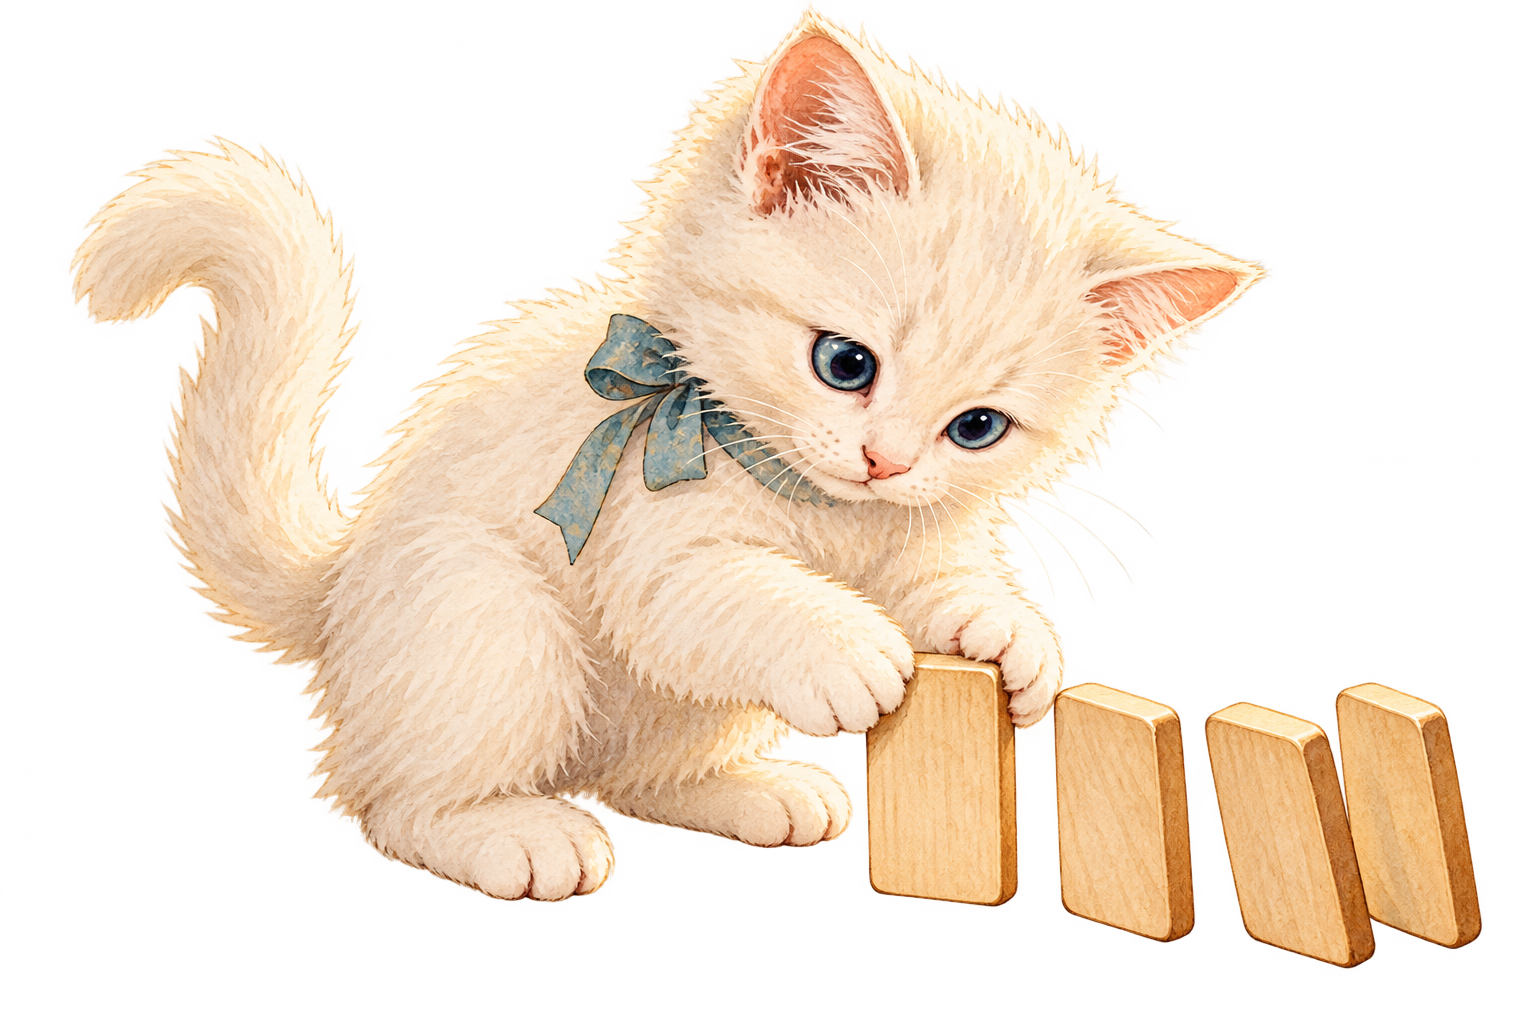
\includegraphics[width=54mm,height=58mm,keepaspectratio]{images/unique/art-72.png}
\label{catflow:72}
\end{wrapfigure}
\textit{Доказательство.} Если \(p\) простое, каждый ненулевой класс имеет представителя \(a\) с \(1\le a<p\). Тогда \(\gcd(a,p)=1\), и по критерию главы \ref{chap:c21} существует обратный к \(a\) по модулю \(p\). Все остальные аксиомы коммутативного кольца уже выполнены.
Если \(m=uv\) составное, где \(1<u,v<m\), классы \([u]_m,[v]_m\) ненулевые, а их произведение \([m]_m\) нулевое. В поле это невозможно по предыдущей теореме. Значит, составной модуль поля не даёт.\hfill\(\blacksquare\)
\par\WFclear\end{minipage}\end{lrbox}%
\ifdim\dimexpr\ht\CatFlowBox+\dp\CatFlowBox\relax<64mm\dp\CatFlowBox=\dimexpr64mm-\ht\CatFlowBox\relax\fi%
\noindent\usebox{\CatFlowBox}\par\addvspace{5pt}

В \(\mathbb F_5\) можно делить на \([2]_5\), умножая на \([3]_5\). В \(\mathbb F_2\) выполнено \([1]_2+[1]_2=[0]_2\). Это не ошибка обычной арифметики, а арифметика другого множества. Упорядочить это поле так, чтобы одновременно сохранились обычные свойства порядка чисел, невозможно: из положительности \(1\) следовала бы положительность \(1+1=0\).

\section{Когда две группы устроены одинаково}
\begin{definition}
\term{Гомоморфизм групп} (group homomorphism) из \((G,*)\) в \((H,\circ)\) — отображение \(\varphi:G\to H\), сохраняющее операцию: \(\varphi(a*b)=\varphi(a)\circ\varphi(b)\). Биективный гомоморфизм называют \term{изоморфизмом} (isomorphism); группы тогда \term{изоморфны} (isomorphic).
\end{definition}

\begin{theorem}[Образ нейтрального и обратного]\label{thm:legacy-c22-7}
Гомоморфизм групп переводит нейтральный элемент в нейтральный и обратный элемент в обратный.
\end{theorem}
\begin{proof}
Пусть \(e_G,e_H\) — нейтральные элементы. Из \(e_G*e_G=e_G\) следует \(\varphi(e_G)\circ\varphi(e_G)=\varphi(e_G)\). Сократим \(\varphi(e_G)\) в группе \(H\); получим \(\varphi(e_G)=e_H\). Далее \(\varphi(a)\circ\varphi(a^{-1})=\varphi(e_G)=e_H\), и аналогичное равенство получается в обратном порядке. Поэтому \(\varphi(a^{-1})\) — обратный к \(\varphi(a)\).
\end{proof}
Пример гомоморфизма: отправить каждое целое число в его класс по модулю \(5\). Сложение сохраняется, но числа \(0\) и \(5\) имеют один образ, поэтому изоморфизма нет. А отображение \(x\mapsto e^x\) задаёт изоморфизм между \((\mathbb R,+)\) и положительными действительными числами с умножением: оно биективно и \(e^{x+y}=e^xe^y\). Формулы экспоненты из главы \ref{chap:c14-exponential} описывают тем самым соответствие двух групп.

\section{Порождающие и знак перестановки}
\begin{definition}
\term{Подгруппа} (\emph{subgroup}) группы \(G\) --- подмножество \(H\), которое содержит единицу и замкнуто относительно умножения и взятия обратного. С тем же действием оно само является группой.
\end{definition}
\begin{definition}
\term{Подгруппа, порождённая множеством} \(S\subseteq G\) (\emph{generated subgroup}), обозначается \(\langle S\rangle\) и состоит из всех конечных произведений элементов \(S\) и их обратных; пустое произведение равно единице. \par\term{Конечно порождённая группа} (\emph{finitely generated group}) --- группа, для которой \(G=\langle S\rangle\) для некоторого конечного \(S\).
\end{definition}
\begin{definition}
\term{Инверсия перестановки} (\emph{inversion}) \(\sigma\in S_n\) --- пара индексов \(i<j\), для которой \(\sigma(i)>\sigma(j)\). \par\term{Знак перестановки} (\emph{sign of a permutation}), имеющей \(N(\sigma)\) инверсий, равен \(\operatorname{sgn}\sigma=(-1)^{N(\sigma)}\). Это чётность перестановки, которую не следует смешивать с чётностью её порядка как элемента группы.
\end{definition}
\begin{theorem}[Мультипликативность знака]\label{thm:olympiad-permutation-sign}
Для перестановок \(\sigma,\tau\in S_n\) выполнено \(\operatorname{sgn}(\sigma\circ\tau)=(\operatorname{sgn}\sigma)(\operatorname{sgn}\tau)\). Знак любой транспозиции равен \(-1\).
\end{theorem}
\begin{proof}
Обмен соседних позиций меняет число инверсий ровно на один: меняется порядок этой пары, а суммарные отношения с прочими позициями сохраняются. Любую перестановку можно отсортировать соседними обменами, каждый раз убирая одну инверсию. Поэтому чётность числа соседних обменов в любом её разложении равна \(N(\sigma)\) по модулю \(2\). При композиции разложения приписываются друг к другу, и их длины складываются; отсюда первая формула. Обмен позиций \(i<j\) можно выполнить \(2(j-i)-1\) соседними обменами; это нечётное число, что доказывает вторую формулу.
\end{proof}

\Needspace{7\baselineskip}\section*{Задачи}
\begingroup\setlength{\parskip}{2pt}
\noindent\begin{minipage}[t]{\linewidth}\textbf{33.1.} Является ли вычитание бинарной операцией на \(\mathbb N_0\)? А на \(\mathbb Z\)?\par\end{minipage}\par
\noindent\begin{minipage}[t]{\linewidth}\textbf{33.2.} Определи, является ли \((\mathbb N_0,+)\) полугруппой, моноидом и группой.\par\end{minipage}\par
\noindent\begin{minipage}[t]{\linewidth}\textbf{33.3.} Образуют ли положительные натуральные числа группу по сложению? Есть ли нейтральный элемент в этом множестве?\par\end{minipage}\par
\noindent\begin{minipage}[t]{\linewidth}\textbf{33.4.} Проверь аксиомы группы для ненулевых рациональных чисел с обычным умножением.\par\end{minipage}\par
\noindent\begin{minipage}[t]{\linewidth}\textbf{33.5.} Почему \((\mathbb Q,\cdot)\) является моноидом, но не группой?\par\end{minipage}\par
\noindent\begin{minipage}[t]{\linewidth}\textbf{33.6.}\starmark{} На \(\mathbb Z\) задано \(a*b=a+b+1\). Найди нейтральный элемент, обратный к \(a\) и проверь, получается ли группа.\par\end{minipage}\par
\noindent\begin{minipage}[t]{\linewidth}\textbf{33.7.} Дай конкретный контрпример ассоциативности операции \(a*b=a-b\) на \(\mathbb Z\).\par\end{minipage}\par
\noindent\begin{minipage}[t]{\linewidth}\textbf{33.8.} Вычисли \(UV\) и \(VU\) для \(U=\begin{pmatrix}1&1\\0&1\end{pmatrix}\), \(V=\begin{pmatrix}1&0\\1&1\end{pmatrix}\). Сделай вывод о коммутативности умножения матриц.\par\end{minipage}\par
\par\addvspace{5pt}\begin{lrbox}{\CatFlowBox}\begin{minipage}[t]{\linewidth}
\setlength{\parskip}{5pt}\setlength{\columnsep}{4.5mm}\setlength{\intextsep}{0pt}
\begin{wrapfigure}[13]{r}{54mm}
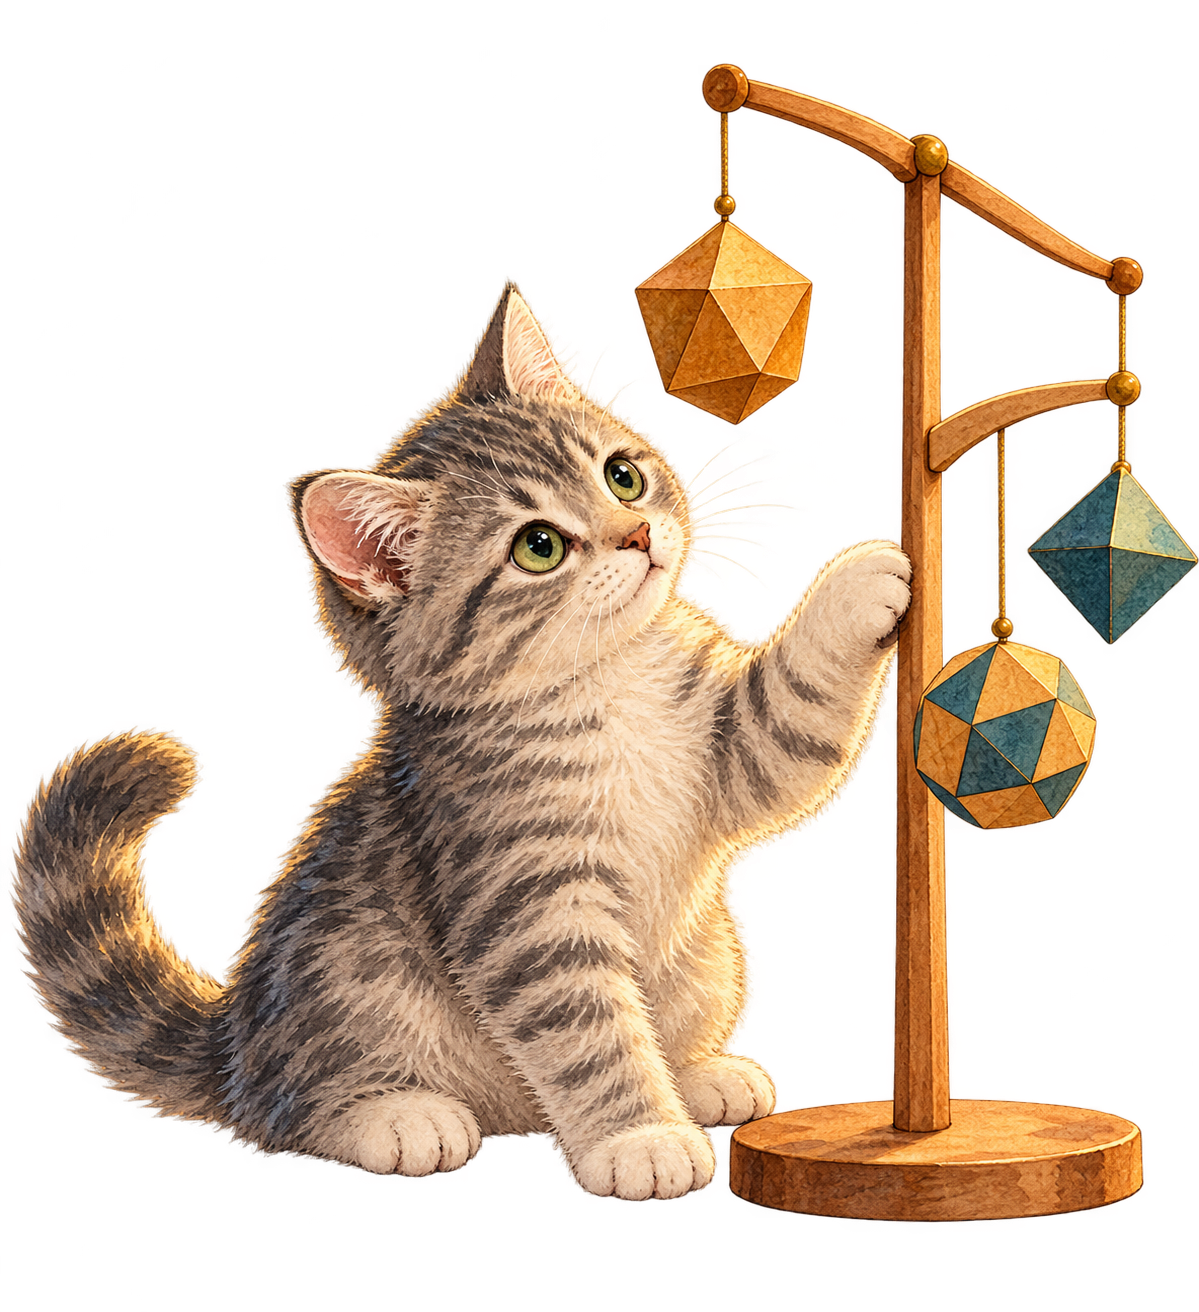
\includegraphics[width=54mm,height=58mm,keepaspectratio]{images/unique/art-65.png}
\label{catflow:65}
\end{wrapfigure}
\textbf{33.9.} Перестановка \(c\) переводит \(1\) в \(2\), \(2\) в \(3\), \(3\) в \(1\). Найди \(c^2,c^3,c^{-1}\), где степень означает композицию.\par

\textbf{33.10.} Квадратную карточку три раза повернули на \(90^\circ\) против часовой стрелки. Какой один поворот даёт тот же результат? Какой поворот отменяет один поворот на \(90^\circ\)?\par

\textbf{33.11.} Робот перемещается по целочисленной прямой. Сдвиг \(T_k\) задаётся \(T_k(x)=x+k\). Найди композицию \(T_8\circ T_{-3}\), нейтральный сдвиг и обратный к \(T_8\).\par

\textbf{33.12.} В недельном расписании действие сдвигает день на \(3\) вперёд. Какое действие его отменяет? На сколько дней вперёд сдвинут три последовательных применения?\par

\textbf{33.13.} Найди все обратимые элементы кольца \(\mathbb Z\). Докажи полноту ответа.\par

\textbf{33.14.} Покажи, что в \(\mathbb Z/6\mathbb Z\) есть ненулевые делители нуля.\par

\textbf{33.15.} В поле \(\mathbb F_5\) найди обратные ко всем четырём ненулевым классам.\par
\par\WFclear\end{minipage}\end{lrbox}%
\ifdim\dimexpr\ht\CatFlowBox+\dp\CatFlowBox\relax<64mm\dp\CatFlowBox=\dimexpr64mm-\ht\CatFlowBox\relax\fi%
\noindent\usebox{\CatFlowBox}\par\addvspace{5pt}

\noindent\begin{minipage}[t]{\linewidth}\textbf{33.16.} Почему \(\mathbb Z/4\mathbb Z\) не поле? Покажи препятствие на одном классе.\par\end{minipage}\par
\noindent\begin{minipage}[t]{\linewidth}\textbf{33.17.} Реши \(2x=1\) в \(\mathbb Z\), в \(\mathbb Q\) и в \(\mathbb F_5\).\par\end{minipage}\par
\noindent\begin{minipage}[t]{\linewidth}\textbf{33.18.} Используя только аксиомы поля, докажи: из \(ab=0\) и \(a\ne0\) следует \(b=0\).\par\end{minipage}\par
\noindent\begin{minipage}[t]{\linewidth}\textbf{33.19.} Проверь, является ли \(\varphi:\mathbb Z\to\mathbb Z/5\mathbb Z\), \(\varphi(n)=[n]_5\), гомоморфизмом по сложению. Инъективен ли он? Сюръективен ли?\par\end{minipage}\par
\noindent\begin{minipage}[t]{\linewidth}\textbf{33.20.} Проверь, задаёт ли \(\varphi(n)=2n\) гомоморфизм \((\mathbb Z,+)\to(\mathbb Z,+)\). Является ли он изоморфизмом?\par\end{minipage}\par
\noindent\begin{minipage}[t]{\linewidth}\textbf{33.21.} Обоснуй, что \(x\mapsto e^x\) — изоморфизм между сложением на \(\mathbb R\) и умножением на положительных действительных числах.\par\end{minipage}\par
\noindent\begin{minipage}[t]{\linewidth}\textbf{33.22.} Докажи единственность нейтрального элемента, не используя числовых примеров.\par\end{minipage}\par
\noindent\begin{minipage}[t]{\linewidth}\textbf{33.23.} Пусть \(b,c\) — двусторонние обратные к \(a\) в моноиде. Докажи \(b=c\), не меняя порядок множителей.\par\end{minipage}\par
\noindent\begin{minipage}[t]{\linewidth}\textbf{33.24.} Редактор сначала удваивает числовую настройку, затем прибавляет \(3\). Сравни это с обратным порядком. Запиши соответствующие композиции \(f(x)=2x\), \(g(x)=x+3\).\par\end{minipage}\par
\noindent\begin{minipage}[t]{\linewidth}\textbf{33.25.}\starmark{} На \(S=\mathbb R\setminus\{-1\}\) задано \(a*b=a+b+ab\). Докажи, что это абелева группа. Найди нейтральный и обратные, используя \(1+(a*b)=(1+a)(1+b)\).\par\end{minipage}\par
\noindent\begin{minipage}[t]{\linewidth}\textbf{33.26.}\starmark{} Реши \(x^2=x\) в произвольном поле и в кольце \(\mathbb Z/6\mathbb Z\). Почему ответы могут различаться?\par\end{minipage}\par
\noindent\begin{minipage}[t]{\linewidth}\textbf{33.27.}\starmark{} Выведи формулу \((a+b)^2=a^2+2ab+b^2\) в коммутативном кольце. Здесь \(2ab=ab+ab\). Какую формулу нужно оставить без коммутативности?\par\end{minipage}\par
\noindent\begin{minipage}[t]{\linewidth}\textbf{33.28.}\starmark{} В \(S_3\) перестановка \(s\) меняет \(1,2\), а \(t\) меняет \(2,3\). Найди \((s\circ t)(1)\) и \((t\circ s)(1)\), затем докажи некоммутативность \(S_3\).\par\end{minipage}\par
\par\Needspace{12\baselineskip}\section*{Олимпиадные задачи}
\par\addvspace{2pt}\begin{lrbox}{\CatFlowBox}\begin{minipage}[t]{\linewidth}
\setlength{\parskip}{2pt}\setlength{\columnsep}{4.5mm}\setlength{\intextsep}{0pt}
\begin{wrapfigure}[11]{l}{54mm}

\includegraphics[width=54mm,height=58mm,keepaspectratio]{images/unique/art-315.png}
\label{catflow:315}
\end{wrapfigure}
\textbf{33.29.}\starmark{} {\small\itshape\href{http://halgebra.math.msu.su/Olympiad/2006/solutions-06.pdf}{Алгебраическая олимпиада МГУ, 2006, № 1}; редакция условия.}\par Каких элементов в группе перестановок \(S_n\) больше: чётного или нечётного порядка? Рассмотри все \(n\ge1\). Порядок элемента — наименьшая положительная степень, дающая единицу.\par

\textbf{33.30.}\starmark{} {\small\itshape\href{https://www.imc-math.org.uk/imc1996/prob_sol.pdf}{IMC, 1996, день 2, № 3}; перевод.}\par Пусть \(G\) — группа обратимых действительных матриц, порождённая \(A=\begin{pmatrix}2&0\\0&1\end{pmatrix}\), \(B=\begin{pmatrix}1&1\\0&1\end{pmatrix}\), а \(H\) — её матрицы с обеими диагональными координатами \(1\). Докажи, что \(H\) — коммутативная подгруппа, которую нельзя породить конечным набором элементов.\par
\par\WFclear\end{minipage}\end{lrbox}%
\ifdim\dimexpr\ht\CatFlowBox+\dp\CatFlowBox\relax<58mm\dp\CatFlowBox=\dimexpr58mm-\ht\CatFlowBox\relax\fi%
\noindent\usebox{\CatFlowBox}\par\addvspace{2pt}

\endgroup
